\section{Вибір скінченнорізницевої схеми. Дискретизація}
\subsection{Попередні зауваження. Оіцінки похідних у рівнянні дифузії за допомогою ряду Тейлора}

Спочатку для демонстрації загальних міркувань розглянемо одновимірне р-ня дифузії
\begin{equation}
\frac{\partial u}{\partial t} = \sigma\frac{\partial^2 u}{\partial^2 x}\label{eq:onedim}
\end{equation}
і отримаємо явний вигляд скінченнорізницевих операторів, якими ми будемо надалі користуватись, з розкладу в ряд Тейлора.

Розклад в ряд Тейлора значення функції $u$ в околі точки $\left(x + \Delta x\right)$, де значення $u(x)$ --- відоме, може бути записано як:
\begin{equation}
u(x+\Delta x) = u(x) +\Delta x\frac{\partial u}{\partial x} + \frac{\Delta x^2}{2}\frac{\partial^2 u}{\partial^2 x} + \frac{\Delta x^3}{6}\frac{\partial^3 u}{\partial^3 x} + O\left(\Delta x^4\right);\label{eq:taylorforw}
\end{equation}
аналогічно для точки $\left(x - \Delta x\right)$: 
\begin{equation}
u(x-\Delta x) = u(x) -\Delta x\frac{\partial u}{\partial x} + \frac{\Delta x^2}{2}\frac{\partial^2 u}{\partial^2 x} - \frac{\Delta x^3}{6}\frac{\partial^3 u}{\partial^3 x} + O\left(\Delta x^4\right)\label{eq:taylorbackw}
\end{equation}
Розв’язуючи \eqref{eq:taylorforw} відносно $\frac{\partial u}{\partial x}$ і опускаючи всі члени вищих порядків, отримуємо
\begin{equation}
\frac{\partial u}{\partial x} = \frac{u(x+\Delta x) - u(x)}{\Delta x} + O\left(\Delta x\right)
\end{equation}
аналогічно для \eqref{eq:taylorbackw} отримуємо
\begin{equation}
\frac{\partial u}{\partial x} = \frac{u(x)-u(x-\Delta x)}{\Delta x} + O\left(\Delta x\right)
\end{equation}
У англомовній літературі останні два вирази прийнято називати \textit{forward і backward difference operator} відповідно. Крім того, віднявши \eqref{eq:taylorbackw} від \eqref{eq:taylorforw} отримаємо центрований різницевий оператор:
\begin{equation}
\frac{\partial u}{\partial x} = \frac{u(x+\Delta x) - u(x-\Delta x)}{2\Delta x} + O\left(\Delta x^2\right),
\end{equation}
який, як бачимо, має вищий порядок точності, ніж два попередні.

Зрештою, додамо \eqref{eq:taylorbackw} і \eqref{eq:taylorforw} й розв’яжемо відносно $\frac{\partial^2 u}{\partial^2 x}$:
\begin{equation}
\frac{\partial^2 u}{\partial^2 x} = \frac{u(x+\Delta x) - 2u(x) + u(x-\Delta x)}{\Delta x^2} + O\left(\Delta x^2\right)
\end{equation}
Тепер \eqref{eq:onedim} може бути переписано як
\begin{equation}
u(t + \Delta t) - u(t) = s_x\left(u(x+\Delta x) - 2u(x) + u(x-\Delta x)\right),
\end{equation}
де $s_x = \frac{\sigma\Delta t}{\Delta x^2}$ --- так зване число дифузії, яке є дуже важливим при оцінці стійкості різницевих схем такого типу.

Нехай тепер потрібно розв’язати \eqref{eq:onedim} на $\left[0,L\right]$ на проміжку часу від $t=0$ до $t=T$ і відомо, що $u(0,x)=u(t,0)=u(t,L) = 0$.
Введемо точки $n\Delta t$, $j\Delta x$, \\
\begin{center}
\vspace{-0.05\linewidth}
$n = 0, \dots\ N$, $j = 0, \dots\ M$ --- цілі числа, $N = T/\Delta t$, $M = L/\Delta x$
\end{center}
і перепишемо \eqref{eq:onedim} згідно з попереднім, використовуючи нові позначення:
\begin{equation}
u^{n+1}_j - u^n_j = s_x\left(u^n_{j+1} -2u^n_j + u^n_{j-1}\right),
\end{equation}
де $u^n_j = u(n\Delta t, j\Delta x)$;
окрім того початкові та граничні умови запишуться як:
\begin{equation}
u^{0}_j = 0, \text{\ }
u^n_0 = u^n_M = 0.
\end{equation}

Подібні міркування, що можуть бути легко відтворені для вищих розмірностей, і приводять якраз до поняття скінченнорізницевих схем як методу числового розв’язання ДРЧП. Замінюючи у постановці конкретної задачі часткові похідні їх наближеннями через
різницеві оператори і обираючи фіксовані кроки $\Delta t$ по часу і $\Delta x \ (\Delta y \dots)$ у просторі (для кожного окремого випадку різницевої схеми кроки можуть бути нерівномірними, змінюватись у процесі розв’язку і т.д.), ми переводимо задачу у скінченновимірний простір --- так звану \textit{сітку}, --- для кожного вузла $j$ якої ми знаходимо розв’язок у деякий момент часу $n$ з отриманих різницевих р-нь, а для точок простору, які не потрапили у сітку, значення може бути відтворене, наприклад, інтерполюванням.

З вищенаведеного також легко бачити, що вибір різницевих операторів, які входять до різницевої схеми, впливає на її порядок точності. Це має велике значення для вибору конкретної схеми для розв’язку тієї чи іншої крайової задачі. Наприклад, для вищерозглянутої схеми порядок точності є $O\left(\Delta t,\ \Delta x^2\right)$. Звичайно доцільним є покращити порядок точності і \textit{стійкість} (про що ще йтиме мова далі), проте це має свою ціну, а саме: ми приходимо до \textit{неявних} cхем, для яких на кожному кроці по часу потрібно розв’язувати СЛАУ (у випадку лінійної однорідної крайової задачі), або ж у більш загальному випадку, якщо не вносити спеціальні корективи, навіть систему нелінійних р-нь.

\newpage
\subsection{Вибір різницевої схеми для р-ня Фішера. Схеми типу Кранка-Ніколсона}
Для підвищення порядку точності було запропоновано багато модификацій найпростішої явної схеми. Детальний огляд і узагальнення у табличному вигляді видів різницевих схем для рівнянь параболічного типу наведено у \cite{richt} (стор. 192-195).
Одним із найбільш розповсюджених є клас неявних схем, який отримується таким чином. Праву частину вихідного р-ня записуємо як суму двох різницевих операторів по просторовим координатам, один з яких береться у точці $n+1$ по часу з вагою $\lambda$, а інший у точці $n$ по часу з вагою $(1-\lambda)$. Явно це виглядає для нашого р-ня \eqref{eq:fisher} так:
\begin{multline}
\frac{\upl{0}{0} - \un{0}{0}}{\Delta t} = \sigma\frac{\lambda(\delta^2_ju)^{n+1}_k + (1-\lambda)(\delta^2_ju)^{n}_k}{\Delta x^2} + \\ + \sigma\frac{\lambda(\delta^2_ku)^{n+1}_j + (1-\lambda)(\delta^2_ku)^{n}_j}{\Delta y^2} + {\lambda (f(u))^{n+1}_{jk} + (1-\lambda)(f(u))^{n}_{jk}} \label{eq:syst}
\end{multline}
де $\left(\delta^2_ju\right)^{n}_k = \un{1}{0} - 2\un{0}{0} + \un{-1}{0}$\ , $f(u)$ --- реактивний логістичний член р-ня \eqref{eq:fisher}.\\
За рахунок такого усереднення похідна по часу де-факто розглядається у точці з індексом $(n+ \frac{1}{2})$, тобто по часу ми маємо записаний у інших позначеннях центрований різницевий оператор, який, як ми бачили, має порядок точності $O\left(\Delta t^2\right)$, отже в цілому даний клас різницевих схем має порядок точності $O\left(\Delta t^2, \Delta x^2, \Delta y^2\right)$.

При $\lambda = \frac{1}{2}$ отримуємо відому схему Кранка-Ніколсона. Загальний ’’шаблон'' для схем цього класу зображений на Рис. 1.
\begin{figure}[h]
\center{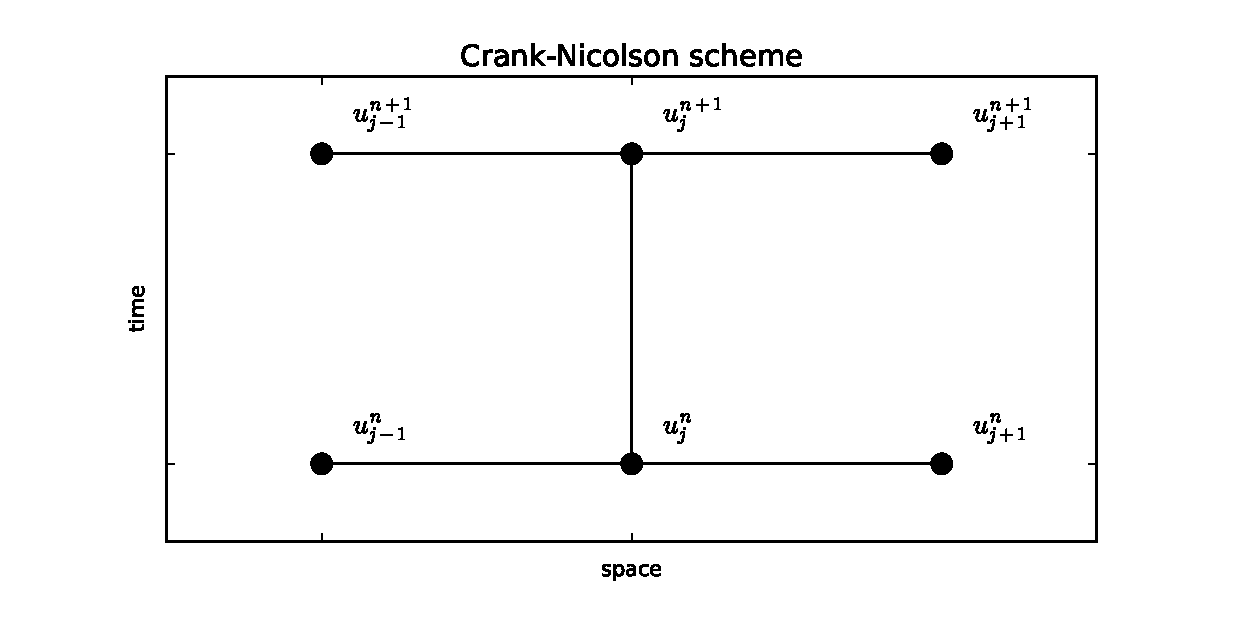
\includegraphics[width=\textwidth]{CNfootprint.eps}}
\caption{}
\label{fig:fig1}
\end{figure} \\
Як неважко бачити, завдяки подібній дискретизації нашого р-ня ми отримуємо на кожному кроці по часу систему р-нь відносно невідомих значень шуканої ф-ї у точках з індексом $(n+1)$, крім того, поки що нелінійних (через квадратичний член). Однак в подальшому ми позбавимось від цієї незручності і використаємо усі переваги даної схеми саме для лінеаризованого випадку. Розмірність такої системи $[(M+1)\times(N+1)]^2$, де $M$ та $N$ --- к-ть вузлів по осям $Ox$ і $Oy$ відповідно, як у прикладі з попереднього пункту. Отже при достатньо маленьких кроках дискретизації розв’язування подібної системи може вимагати багато обчислювальних ресурсів;
тим не менше, у лінійному випадку така система є дуже розрідженою і  має разом з граничними умовами (які в даному випадку представлені у формі Дирихле) чітко виражений 5-діагональний вид, що дозволяє нам використовувати оптимізовані формати збереження і методи розв’язання розріджених систем.

\subsection{Лінеаризація отриманої системи}
Як уже було вказано, якщо використовувати для дисткретизації \eqref{eq:fisher} схему типу Кранка-Ніколсона у її стандартному вигляді, то отримана система р-нь \eqref{eq:syst} є нелінійною, що призводить до суттєвих незручностей з обчислювальної точки зору (необхідності використовувати своєрідні, більш складні ніж для розріджених матриць, формати збереження, виключно ітераційні алгоритми розв’язку, накшталт Ньютона-Рафсона, або метод Крилова оптимізації вектор-функцій багатьох змінних, які вимагають обчислень якобіанів порядку (для нашого випадку) $[(M+1)\times(N+1)]^4$, що вимагає ресурсів ще більше, ніж зберігання 5-діагональної розрідженої матриці у звичайному ``densed'' вигляді). Тому нами запропоновано дещо інший підхід, який базується на зведенні вже отриманої системи до лінійного вигляду.

Нелінійність у \eqref{eq:syst} вносить квадратичний член $\left(\upl{0}{0}\right)^2$, отже зводити до лінійного вигляду будемо саме його. Розглянемо похідну за часом від функції $u^2(t,x,y)$:
\begin{equation}
\frac{\partial\left(u^2\right)}{\partial t} = 2u\frac{\partial u}{\partial t}
\end{equation}
що, використовуючи апроксимацію різницевим оператором по часу, може бути переписано як
\begin{equation}
\frac{\left(u^2\right)^{n+1}_{jk} - \left(u^2\right)^{n}_{jk}}{\Delta t} = \frac{2u^n_{jk}\left(u^{n+1}_{jk} - u^n_{jk}\right)}{\Delta t}
\end{equation}
звідки маємо
\begin{equation}
\left(u^{n+1}_{jk}\right)^2 = \left(u^{n}_{jk}\right)^2 + 2u^n_{jk}\left(u^{n+1}_{jk} - u^n_{jk}\right)
\end{equation}
де величини у правій частині на кожному кроці по часу відомі.
Тепер вводячи позначення $\omega_{jk} = \left(\upl{0}{0} - \un{0}{0}\right)$ і записуючи граничні (за постановкою задачі значення на границі --- константніпо часу) умови
\begin{equation}
\omega_{0,k} = \omega_{M,k} = \omega_{j,0} = \omega_{j,N} = 0
\end{equation}
ми приходимо до лінеаризованого варіанту системи \eqref{eq:syst}, яка тепер є 5-діагональною СЛАУ. Розв’язуючи її на кожному кроці відносно $\omega_{jk}$ і покладаючи $\upl{0}{0} = \omega_{jk} + \un{0}{0}$ приходимо до розв’язку початкової задачі.
